%% Preamble %%
\documentclass[paper=a4]{article}

\usepackage{float}
\usepackage{geometry}
\geometry{verbose,tmargin=2.25cm,bmargin=2cm,lmargin=2.25cm,rmargin=2cm}
\geometry{a4paper}
\usepackage{multirow}


\usepackage[T1]{fontenc}
\usepackage{fourier}
\usepackage[utf8]{inputenc}
\usepackage[spanish]{babel}				

\usepackage{amsmath,amsfonts,amsthm} % Math packages
\usepackage[pdftex]{graphicx}	

\makeatletter
%%%%%%%%%%%%%%%%%%%%%%%%%%%%%% User specified LaTeX commands.
\usepackage{fancyhdr}
\usepackage{lscape}
\pagestyle{fancy}
\lhead{Electr\'onica II 22.12}
\chead{TPL1}
\rhead{ITBA}
\renewcommand{\headrulewidth}{1pt}
\renewcommand{\footrulewidth}{1pt}

\makeatother

\usepackage{babel}
\addto\shorthandsspanish{\spanishdeactivate{~<>}}

\begin{document}

\tableofcontents
\newpage

\section{Objetivos - Parámetros del sistema}

En el presente trabajo práctico se realiza el diseño e implementación de un amplificador de audio de un solo canal, con las siguientes especificaciones:

\begin{center}
\begin{tabular}{|c|c|}
\hline 
$PO_{MAX}[W]$ & $Z_{IN}[\Omega]$\\
\hline 
\hline 
$22$ & $50K$\\
\hline 
\end{tabular}
\end{center}

La carga nominal para el diseño considerada es de $8\Omega$, y se trabajará en el rango de frecuencias de audio. Es decir, en la banda de 20Hz a 20KHz.

\section{Diseño del sistema}

El circuito propuesto es un amplificador con salida diferencial, utilizando etapas de potencia clase AB con simetría complementaria. El circuito simplificado se muestra a continuación.

\begin{figure}[!ht]
\begin{centering}
%\includegraphics[scale=0.32]{Imagenes/CircuitoSinCap.png}
\par\end{centering}
\caption{Circuito amplificador con salida diferencial (simplificado)}
\end{figure}

Para tener un cierto margen a las especificaciones propuestas, se diseñará para una potencia de $25W$ sobre la carga.

\subsection{Etapa de salida}

El circuito en cuestión es algo no tan común dado que la salida no está referida a masa, sino que la misma es diferencial. En la figura se muestra centralmente la etapa de salida para analizar.

\begin{figure}[!ht]
\begin{centering}
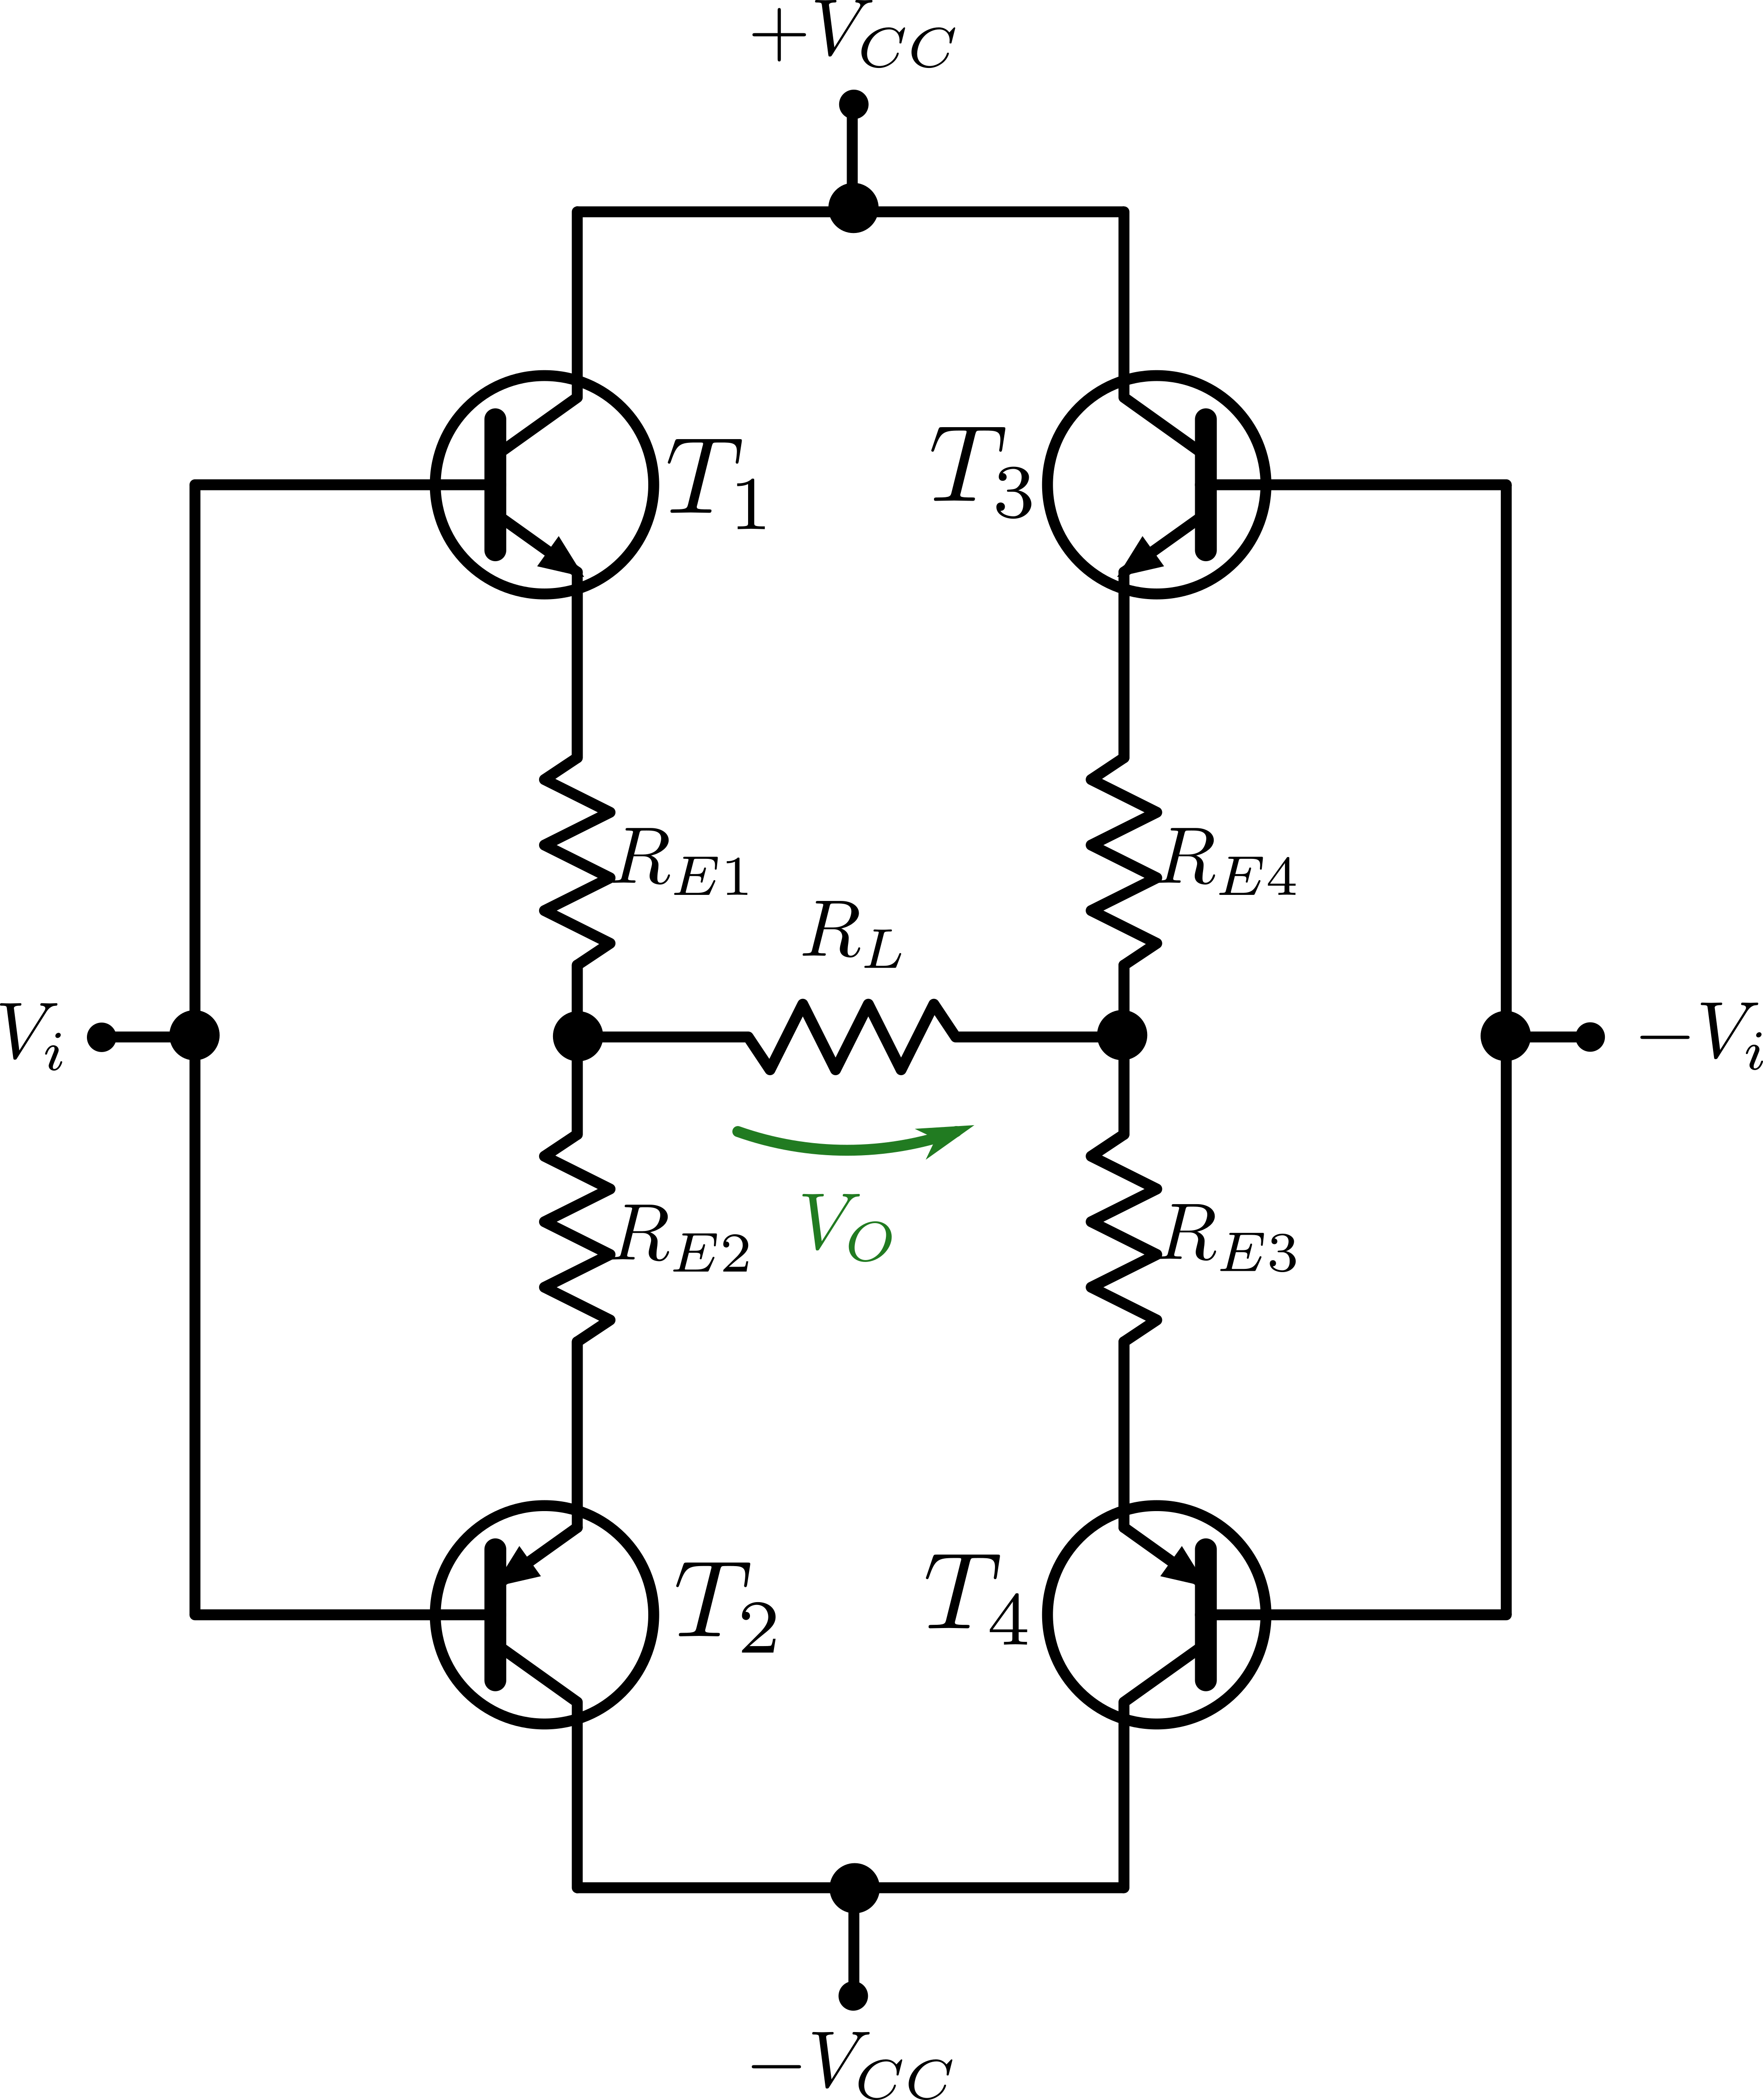
\includegraphics[scale=0.5]{Imagenes/EtapaSalida.png}
\par\end{centering}
\caption{Etapa de salida diferencial}
\end{figure}

Teniendo la potencia buscada sobre la carga, se puede realizar el diseño del amplificador desde ``afuera hacia adentro'' (es decir, desde la salida hacia el generador de entrada). Considerando para el diseño que $P_{O_{MAX}} = 25W$, se calcula la $\hat{V_O}_{MAX}$ necesaria:

\[
P_{O_{MAX}} = \frac{{\hat{V_O}_{MAX}}^2}{2R_L} \Longrightarrow \hat{V_O}_{MAX} = \sqrt{2 \cdot R_L \cdot P_{O_{MAX}}} = 20V
\] 

Dicha tensión sería la tensión pico máxima diferencial sobre la carga. Tomando uno de sus bornes respecto de masa, es la mitad del valor, es decir $\frac{\hat{V_O}_{MAX}}{2} = 10V$.\par
Con la tensión calculada, se puede obtener la $\hat{I_O}_{MAX}$ sobre la carga:

\[
\hat{I_O}_{MAX} = \frac{\hat{V_O}_{MAX}}{R_L} = 2.5A
\]

Unos transistores de potencia adecuados a estas especificaciones son los darlington complementarios TIP122 (NPN) y TIP127 (PNP). Por lo que se seleccionan $T_1 = T_3 = \textrm{TIP122}$ y $T_2 = T_4 = \textrm{TIP127}$. 

%FALTA REVISAR LA EXPLIACION ESTA!!!

Esta implementación presenta algunas ventajas respecto de una con salida referida a masa. En el caso de este último (correspondería tomar solo una de las dos mitades del circuito), cada fuente de alimentación aporta corriente en uno de los dos semiciclos de señal (dado que en cada semiciclo conduce solo uno de los dos transistores NPN o PNP), mientras que en la implementación propuesta ambas fuentes proporcionan corriente en ambos semiciclos. En el semiciclo positivo (es decir, tomando $V_i > 0$) conducen los transistores $T_1$ y $T_4$, mientras que en el negativo conducen $T_2$ y $T_3$. Esta configuración es conocida como ``Puente H'', la cual es común implementarla en el control de sentido de giro de un motor (siendo el motor la carga $R_L$).\par
Se considera nuevamente:

\[
P_{O_{MAX}} = \frac{{\hat{V_O}_{MAX}}^2}{2R_L}
\]

Para observar una de las ventajas de esta implementación, se toma medio circuito (como se mencionó anteriormente), diseñándolo para una cierta potencia $P_{O_{MAX}}$, que dará lugar a una $\hat{V_O}_{MAX}$. El otro hemicircuito será similar pero con una fase de $180^{\circ}$. Conectando la carga $R_L$ entre ambas salidas, en cada terminal de la misma se tendría entonces $V_O$ y $-V_O$ respectivamente. Esto quiere decir que sobre la carga se tendría una diferencia de tensión de $2V_O$. Si se reemplaza en la ecuación de potencia anterior, resulta que la $P_{O_{MAX}}$ en el circuito propuesto es cuatro veces mayor que para el mismo diseño sobre un circuito con salida referida a masa, utilizando fuentes de alimentación de igual valor de tensión en ambos casos (pero las fuentes deberán ser del doble de potencia para el circuito diferencial).\par
Se detalla el cálculo de las potencias en la sección de cálculo de protección térmica con disipador.

\subsection{Fuente de corriente $I_F$}

Para las fuentes de corriente $I_F$ expresadas en el diseño, se implementó el siguiente circuito:

\begin{figure}[!ht]
\begin{centering}
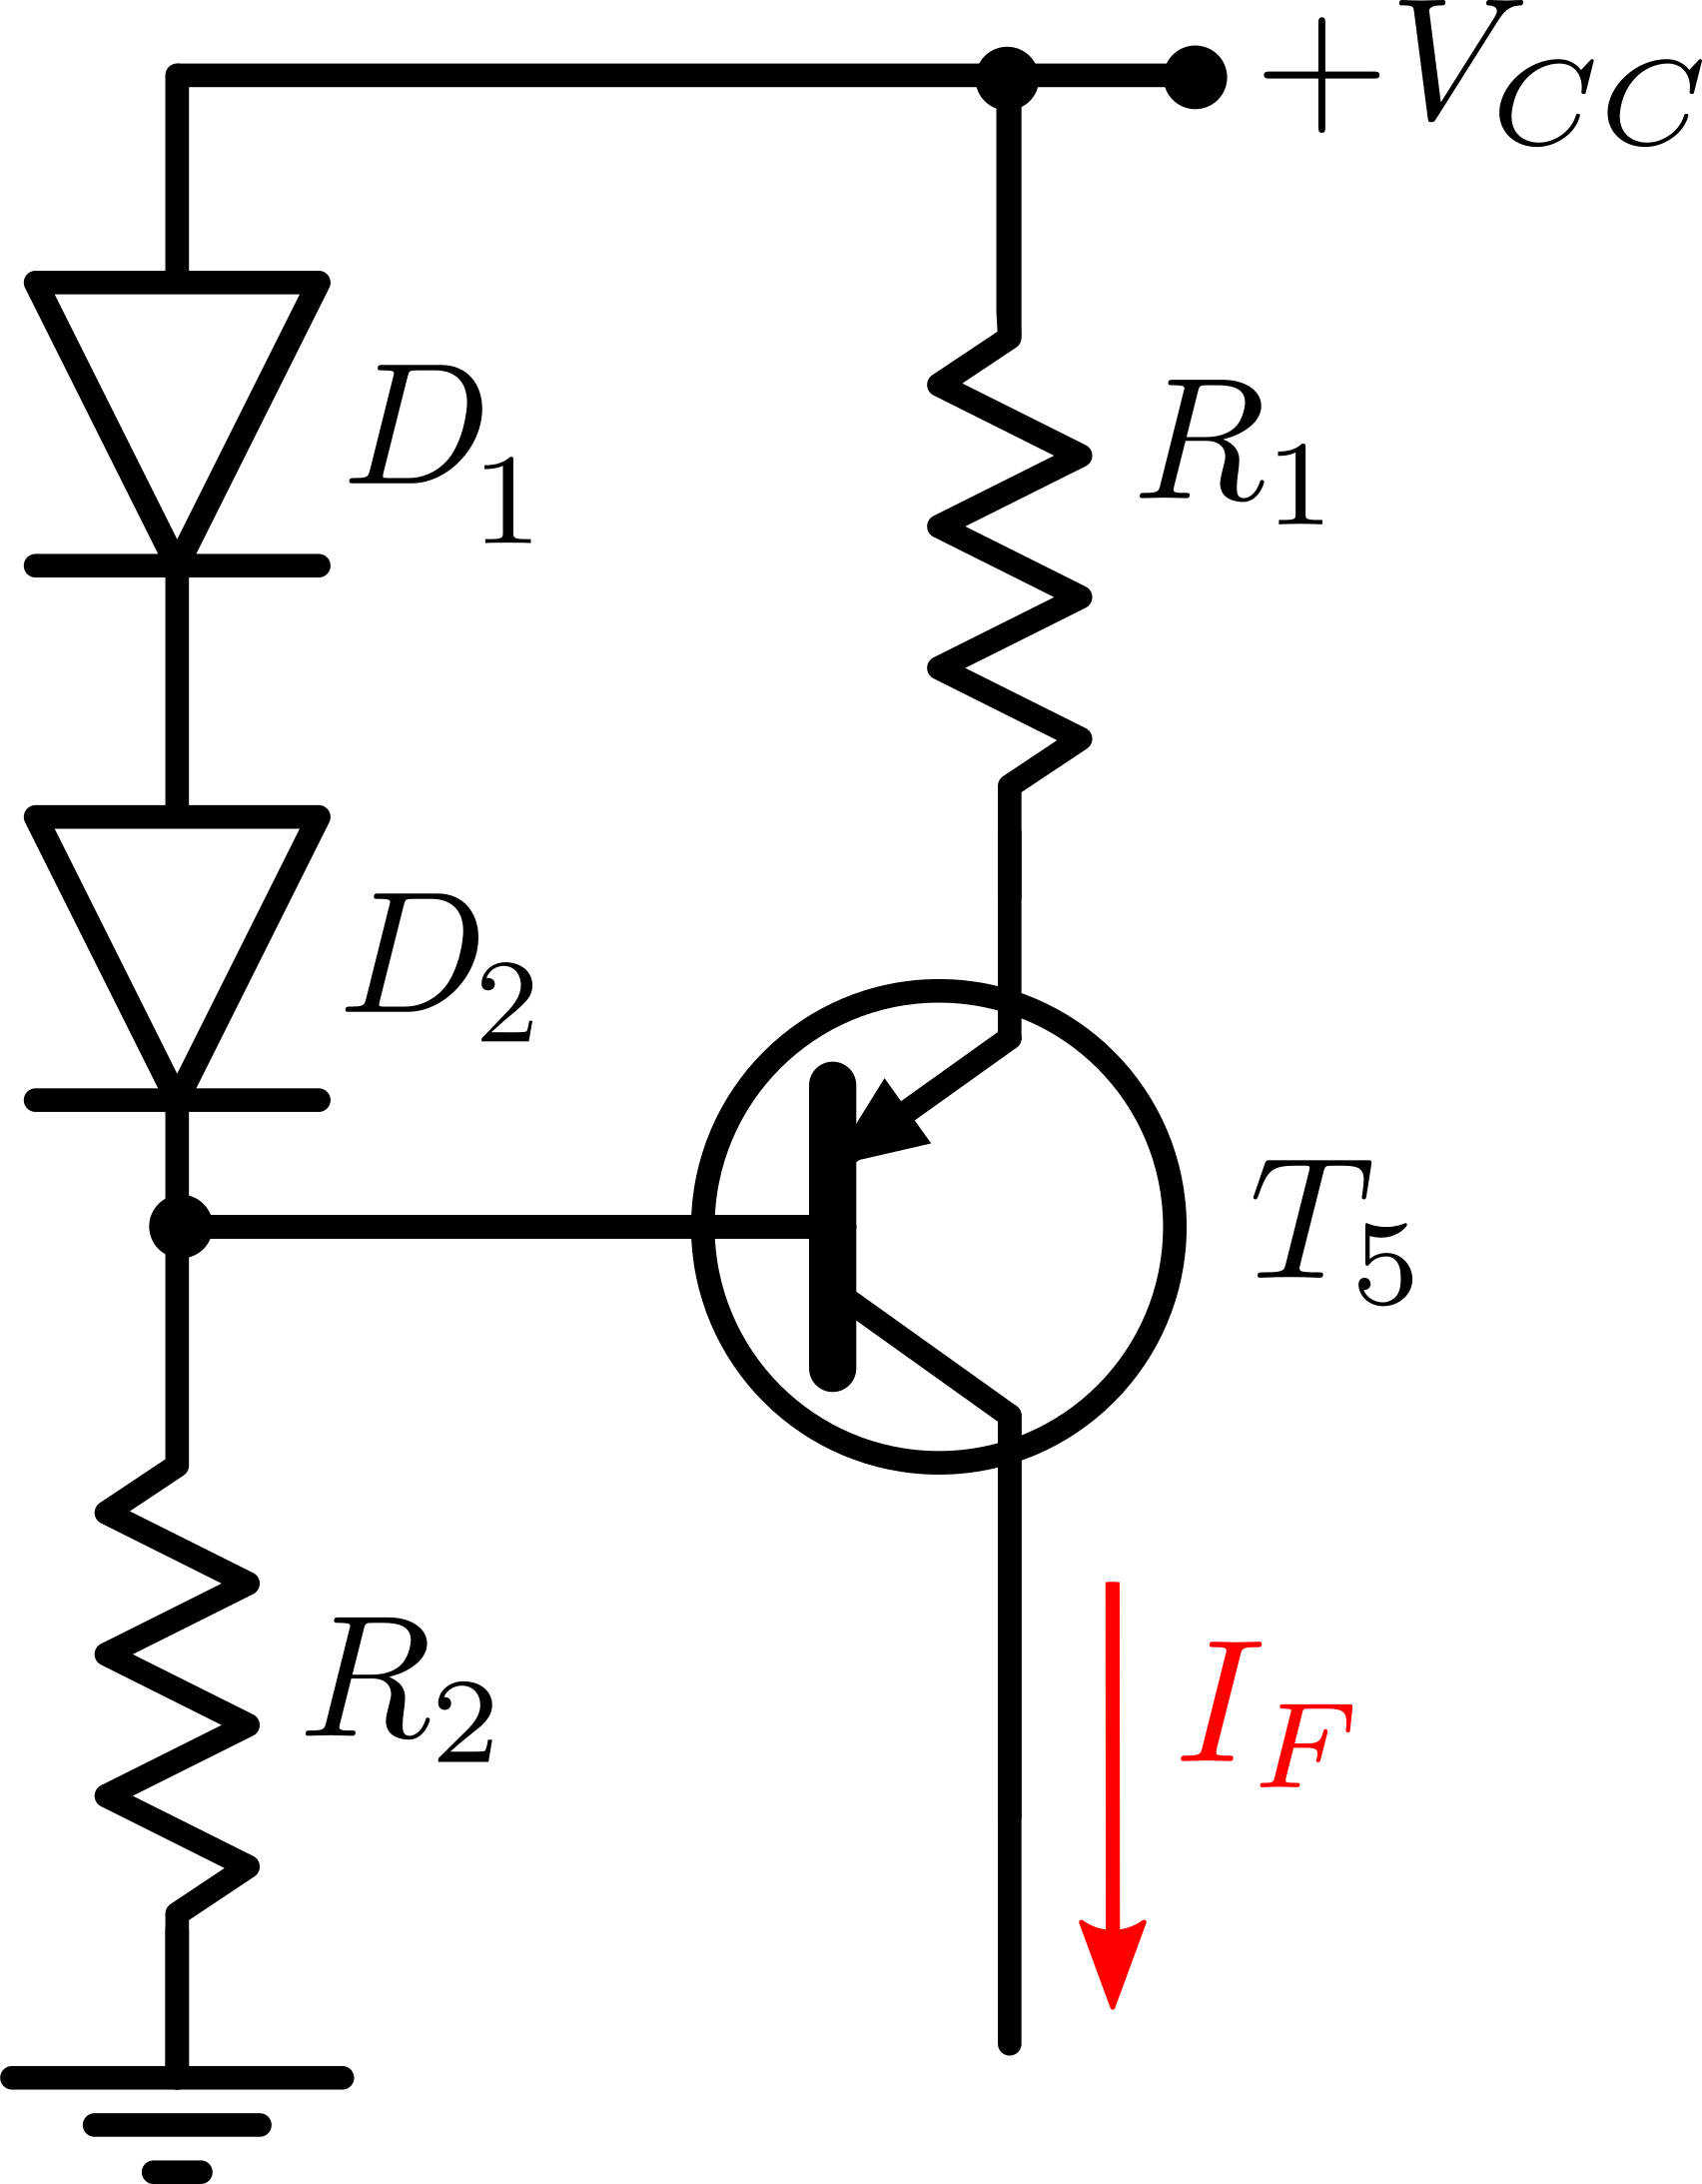
\includegraphics[scale=0.5]{Imagenes/FuenteIF.png}
\par\end{centering}
\caption{Fuente de corriente}
\end{figure}

Dado que la función de los diodos $D_1$ y $D_2$ es solamente provocar una caída de tensión similar a la $V_{BE5_{ON}}$, se utilizan los comunes 1N4148. Considerando que $R_2$ permite polarizarlos correctamente, se tiene recorriendo la malla:

\[
V_{D2} + V_{D1} - I_F \cdot R_1 - V_{BE5_{ON}} = 0
\]

Considerando $V_{D1} = V_{D2} = V_{BE5_{ON}} = V_D = 0.7V$, se tiene:

\[
I_F \cdot R_1 = V_D \Longrightarrow R_1 = \frac{V_D}{I_F}
\]

Del diseño de la etapa de potencia se obtuvo que $\hat{I_O}_{MAX} = 2.5A$. Considerando que los transistores TIP utilizados poseen un $HFE_{MIN} = 1000$ según la hoja de datos (ON Semiconductor), se calcula la corriente de base mínima necesaria que deberá poder proveerles la fuente de corriente (tomando de referencia al transistor $T_1$):

\[
\left. I_{B1_{MIN}} \right|_{I_{O_{MAX}}} = \frac{\hat{I_O}_{MAX}}{HFE_{MIN}} = 2.5mA \Longrightarrow I_{F_{MIN}} = 2.5mA
\]

Entonces se tiene:

\[
R_{1_{MAX}} = \frac{V_D}{I_{F_{MIN}}} = 280\Omega \Longrightarrow R_1(N) = 270\Omega
\]

Se normaliza hacia abajo para asegurar la $I_{F_{MIN}}$.

\end{document}
